\section{Results}

Does MI increase with accuracy on validation set? Does it increase with training time?


In total, \red{these model where trained}. The average runtime for training is \red{insert average runtime}. 

Figures~\cref{fig:train_val_bottle_4,fig:train_val_bottle_6,fig:train_val_bottle_15,fig:train_val_bottle_16} show the training and validation losses for each ensemble the model was trained on. Vertical lines indicate the epoch with best validation performance. \red{Quantify epoch range with best validation performance.} Each model then reaches a plateau \red{in epoch range...} \red{Does this epoch range change across bottleneck dimensions? I.e. were does model take longer to learn?}

In the following, two sources of error in the MI estimation will be discussed. The error of the MI estimation from one training run, stemming from the variability of log probability values on the test set, will be referred to as the \textit{model error}. The error of the MI estimation stemming from different weight initializations, i.e. seeds, will be referrred to as the \textit{seed error}.

One observes a higher seed variance for models with smaller bottleneck dimensions. There is also a higher variability in their training and validation losses across seeds. \red{Quantify the seed variance for best validation loss here.} This indicates a higher training instability for models with smaller bottleneck dimension.
\begin{figure}
    \centering
    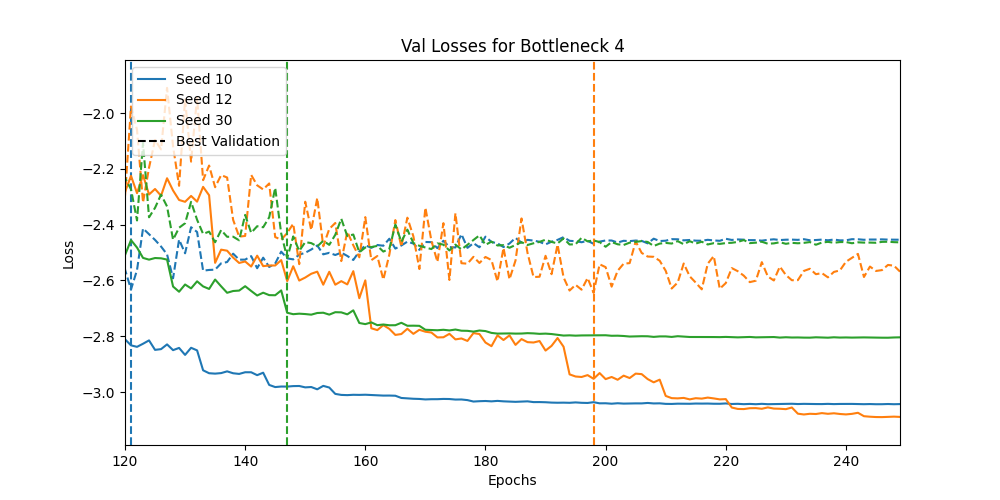
\includegraphics[width=\linewidth]{graphics/ensemble_4/joint_losses.png}
    \caption{Train and Validation Losses for Bottleneck Dimension 4}
    \label{fig:train_val_bottle_4}
\end{figure}
\begin{figure}
    \centering
    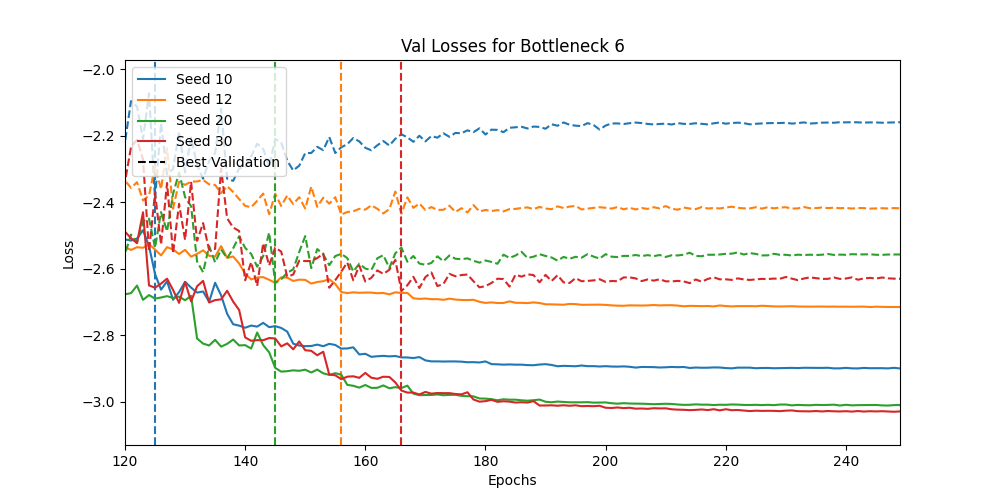
\includegraphics[width=\linewidth]{graphics/ensemble_6/joint_losses.png}
    \caption{Train and Validation Losses for Bottleneck Dimension 4}
    \label{fig:train_val_bottle_6}
\end{figure}
\begin{figure}
    \centering
    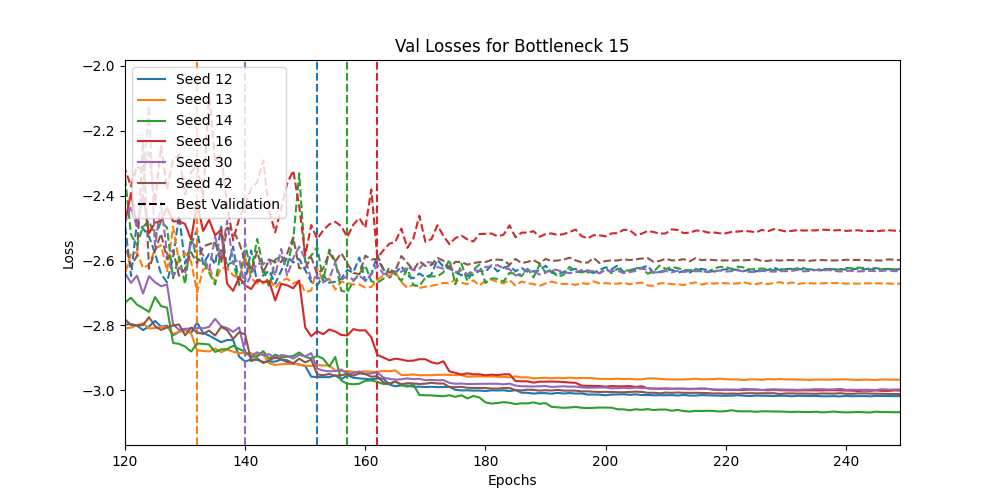
\includegraphics[width=\linewidth]{graphics/ensemble_15/joint_losses.png}
    \caption{Train and Validation Losses for Bottleneck Dimension 4}
    \label{fig:train_val_bottle_15}
\end{figure}
\begin{figure}
    \centering
    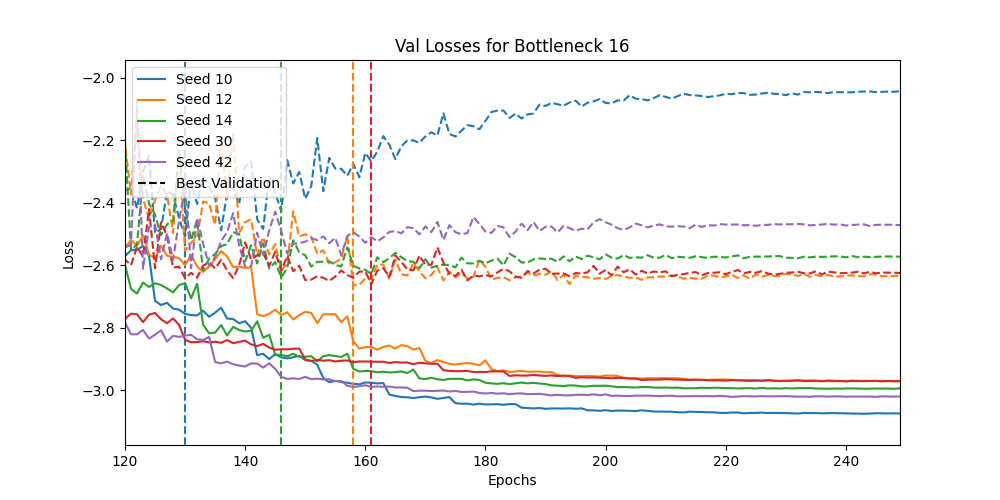
\includegraphics[width=\linewidth]{graphics/ensemble_16/joint_losses.png}
    \caption{Train and Validation Losses for Bottleneck Dimension 4}
    \label{fig:train_val_bottle_16}
\end{figure}

% \begin{figure}[]
%     \centering
%     \begin{subfigure}{0.49\textwidth}
%         \centering
%         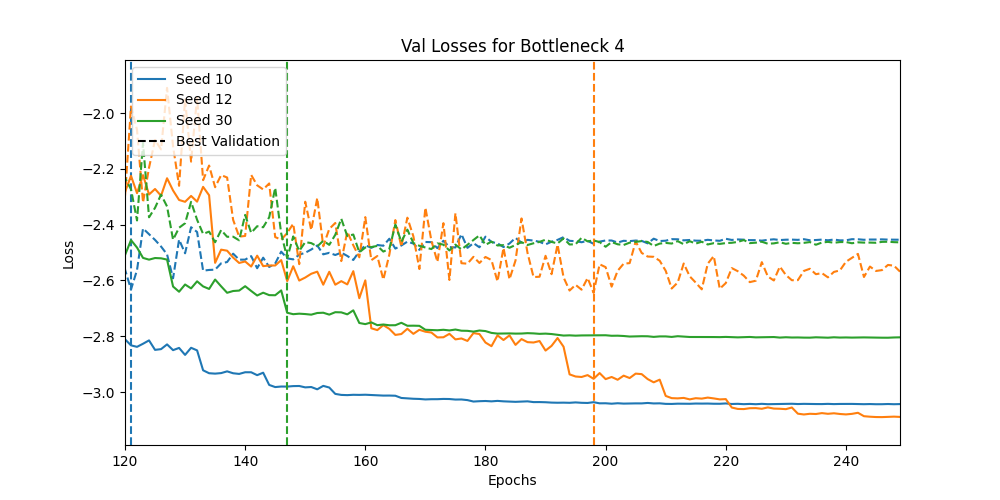
\includegraphics[width=\linewidth]{graphics/ensemble_4/joint_losses.png}
%         \caption{caption}
%         \label{fig:ensemble_4_joint_losses}
%     \end{subfigure}
%     \hfill
%     \begin{subfigure}{0.49\textwidth}
%         \centering
%         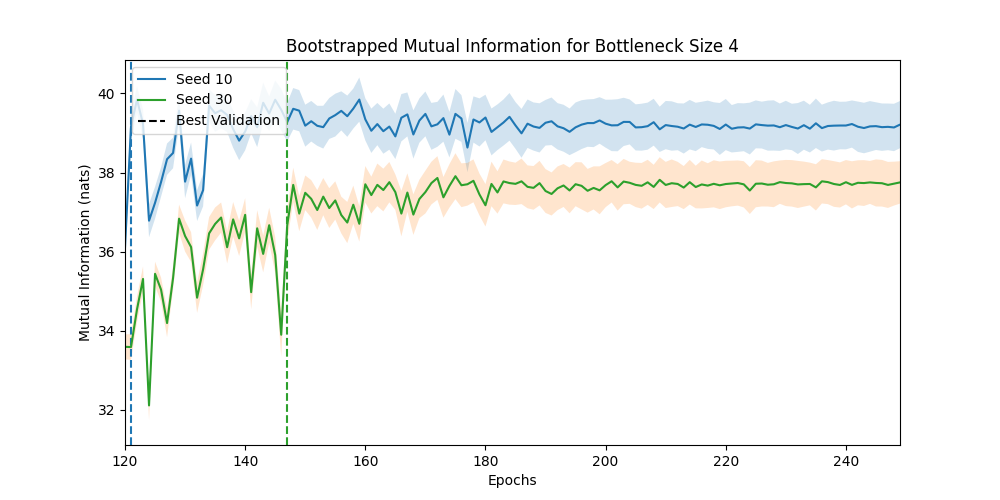
\includegraphics[width=\linewidth]{graphics/ensemble_4/mutual_information_bootstrapped.png}
%         \caption{caption}
%         \label{fig:ensemble_4_ce}
%     \end{subfigure}

%     \vspace{0.5cm}

%     \begin{subfigure}{0.49\textwidth}
%         \centering
%         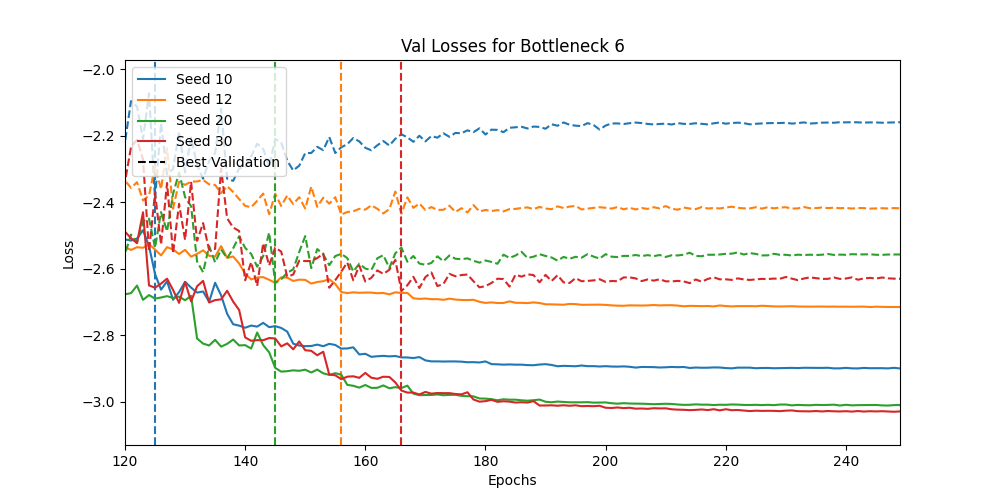
\includegraphics[width=\linewidth]{graphics/ensemble_6/joint_losses.png}
%         \caption{Bottom left}
%         \label{fig:ensemble_6_joint_losses}
%     \end{subfigure}
%     \hfill
%     \begin{subfigure}{0.49\textwidth}
%         \centering
%         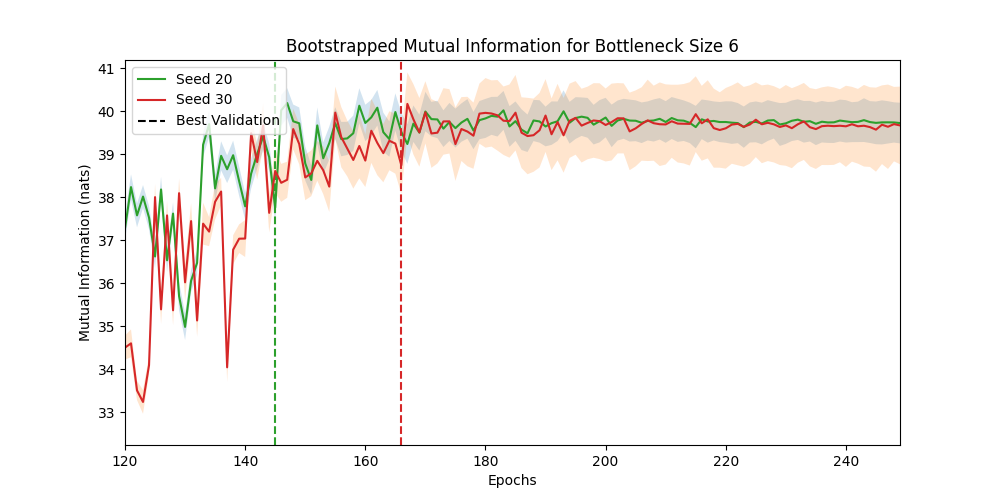
\includegraphics[width=\linewidth]{graphics/ensemble_6/mutual_information_bootstrapped.png}
%         \caption{Bottom right}
%         \label{fig:ensemble_6_ce}
%     \end{subfigure}

%     \caption{Overall caption for both figures}
% \end{figure}


Figures~\cref{fig:mi_bootstrap_bottle_4,fig:mi_bootstrap_bottle_6,fig:mi_bootstrap_bottle_15,fig:mi_bootstrap_bottle_16} show the estimated conditional entropy per epoch for each ensemble the model was trained on. Vertical lines again mark the epoch with best validation performance. All models reach a saturated estimate of the conditional entropy \red{in the epoch range...} The conditional entropy curves showcase a higher instability than the validation curves, which is attributed to the smaller size of the test set.

The model error on the conditional entropy estimate grows with increasing training steps. Some reionization histories are attributed with very low likelihood, such that the distribution of $\log q_\theta (\text{label}_i|\text{summary}_i)$ has a heavy left-sided tail. This is in parts because of the distribution of the labels themselves. 

A separate normalizing flow is trained on the label distribution. \red{Discuss other possible modelling choices and why not took them} The model with best validation performance is chosen for the following analysis. It's distribution of $\log \tilde{q}_\theta (\text{label}_i)$ also showcases a heavy left-sided tail. 

As an example, a histogram plot of the distributions $\log q_\theta (\text{label}_i|\text{summary}_i)$ and $\log \tilde{q}_\theta (\text{label}_i)$ is shown in figure~\red{insert figure}. 

According to the CLT, one would estimate the model error by the standard deviation. The heavy kurtosis inflates the value of standard deviation. As an alternative estimate of error, a bootstrapping method is implemented. \red{Quote some source that cites this as best practice.} \red{The exact values used for bootstrapping for reproducibility.} \red{Something on interpretation of bootstrap results.}

\begin{figure}
    \centering
    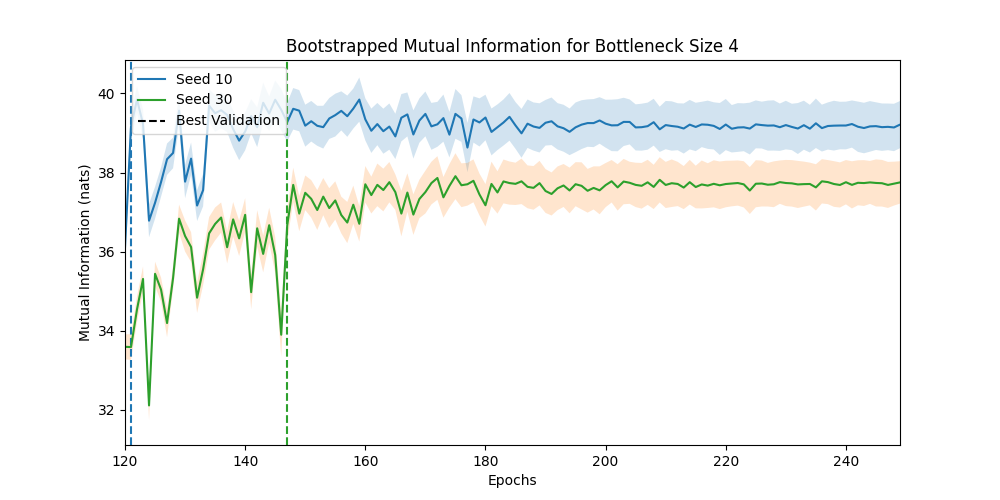
\includegraphics[width=\linewidth]{graphics/ensemble_4/mutual_information_bootstrapped.png}
    \caption{Mutual Information per Epoch for Bottleneck Dimension 4}
    \label{fig:mi_bootstrap_bottle_4}
\end{figure}
\begin{figure}
    \centering
    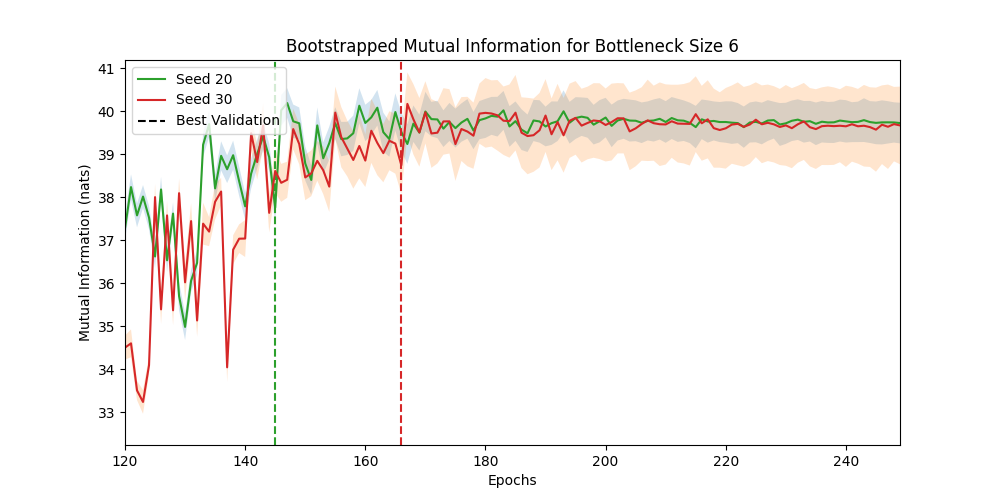
\includegraphics[width=\linewidth]{graphics/ensemble_6/mutual_information_bootstrapped.png}
    \caption{Mutual Information per Epoch for Bottleneck Dimension 4}
    \label{fig:mi_bootstrap_bottle_6}
\end{figure}
\begin{figure}
    \centering
    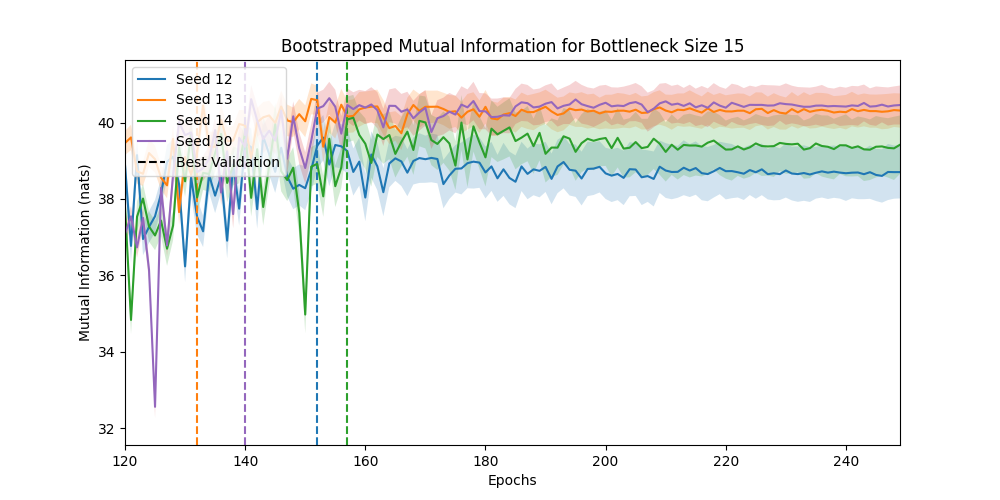
\includegraphics[width=\linewidth]{graphics/ensemble_15/mutual_information_bootstrapped.png}
    \caption{Mutual Information per Epoch for Bottleneck Dimension 4}
    \label{fig:mi_bootstrap_bottle_15}
\end{figure}
\begin{figure}
    \centering
    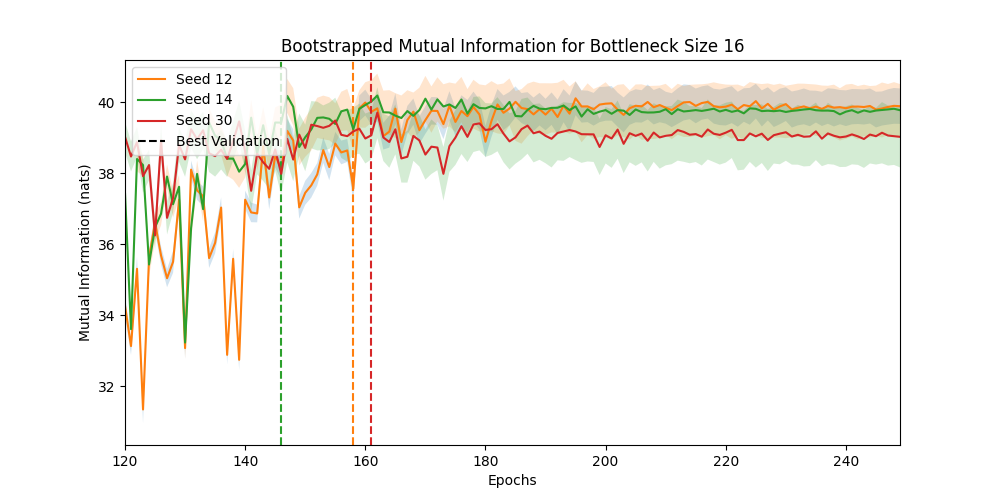
\includegraphics[width=\linewidth]{graphics/ensemble_16/mutual_information_bootstrapped.png}
    \caption{Mutual Information per Epoch for Bottleneck Dimension 4}
    \label{fig:mi_bootstrap_bottle_16}
\end{figure}

For each bottleneck dimension, the final MI estimate is made by selecting the model with best validation loss from each seed and 

averaging the conditional entropy for each of these models. The final error on the CE estimate is comprised of the model error and the \text{seed error}, stemming from the variability of results across different seeds. The final estimates with errors as shown in table~\ref{tab:CE_results}.
\begin{table}[htbp]
\centering
\caption{Final Esimation of CE per Bottleneck Dimension (all entropy values in~\si{nats})}
\label{tab:CE_results}
\begin{tabular}{l c c c c}
\toprule

Bottleneck & CE & Seed error & Model error & No. samples\\
\midrule
4 & $38.81\pm 0.71$ & $0.39$ & $0.12$ & $3$ \\
6 & $38.49\pm 0.95$ & $0.83$ & $0.06$ & $4$ \\
15 & $39.90\pm 0.42$ & $0.13$ & $0.05$ & $5$ \\
16 & $39.57\pm 0.46$ & $0.13$ & $0.09$ & $4$ \\

\bottomrule
\end{tabular}
\end{table}
These results can be described as follows: One does observe a general trend of increasing mutual information for increased bottleneck dimension, though the increase is not monotonous. In all cases, the seed error is larger than the model error, indicating training instablity to be the largest source of error in this setup. 

\red{This indicates the seed error being overestimated? Maybe have to exclude some model. Talk about decision mechanisms and how this introduces bias}

\red{Results if including selection bias}